 \providecommand{\main}{../../..}
\documentclass[\main/main.tex]{subfiles}
\begin{document}
\subsection{Esercizio 1}
Dato il seguente problema di PL:

\begin{figure}
  \begin{align*}
    \max z = x_1 + x_2   \\
    x_1 - 3x_2  & \leq 9 \\
    -x_1 - 3x_2 & \geq 6 \\
    x_1 - x_2   & \geq 0 \\
    x_1         & \leq 1 \\
    x_1         & \in \R \\
    x_2         & \leq 0
  \end{align*}
  \caption{Esercizio 1}
\end{figure}

\begin{enumerate}
  \item Si disegni la regione ammissibile e si evidenzi il vertice ottimo per via grafica, riportando il valore di z e di tutte le variabili del modello.
  \item Si ricavi per via grafica per quali valori di $c_1$, ora pari a $1$, la \textbf{composizione} della base ottima non cambia.
  \item Si risolva mediante gli scarti complementari il duale del problema.
\end{enumerate}

\subsection{Soluzione esercizio 1}

\subsubsection*{Identifico soluzione ottima}

\begin{figure}
  \begin{subfigure}{0.49\textwidth}
    \xygraph{-4.5}{1}{-4.5}{-1.5}{-9}{x-3*y<=9&&-x-3*y>=6&&x-y>=0}{x+y}
    \caption{Il vertice ottimo ha coordinate $\bmx = \rnd{1, -\frac{7}{3}}$}
  \end{subfigure}
  \begin{subfigure}{0.49\textwidth}
    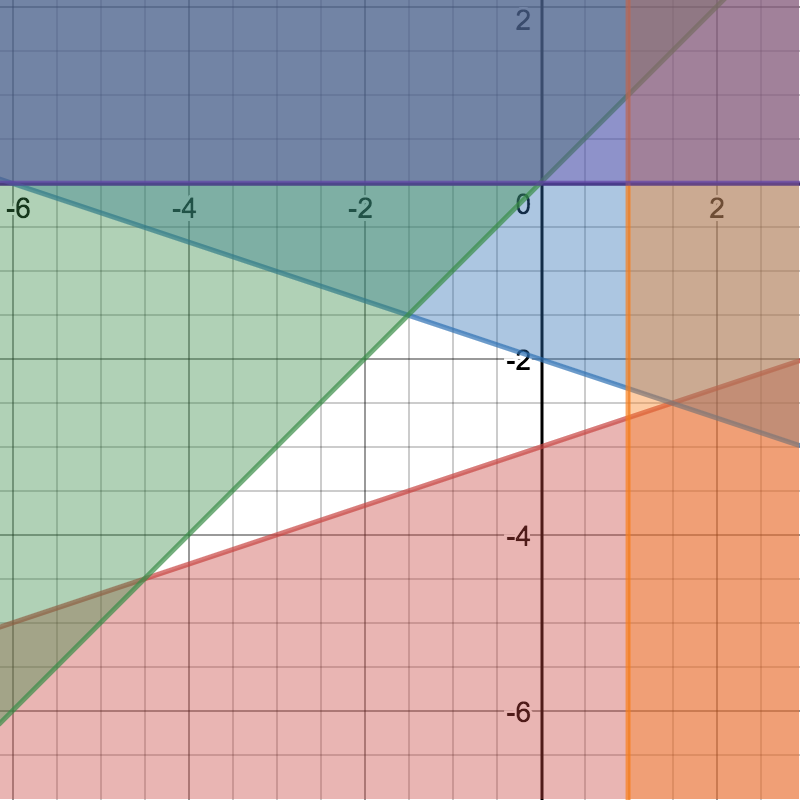
\includegraphics[width=0.9\textwidth]{2016_09_05}
    \caption{Regione di ammissibilità del problema}
  \end{subfigure}
  \caption{Vertice ottimo del problema}
\end{figure}

\subsubsection*{Riporto variabili}

\begin{align*}
  z   = -\frac{4}{3},\quad
  x_1 = 1           ,\quad
  x_2 = -\frac{7}{3},\quad
  s_1 = 1           ,\quad
  s_2 = 0           ,\quad
  s_3 = \frac{10}{3},\quad
  s_4 = 0
\end{align*}
\subsubsection*{Determino il valore di $c_1$}
Il vertice verso cui posso spostarmi abbassando il valore di $c_1$ è quello identificato dall'intersezione di $v_3$ e $v_2$.

Il vertice più ``vicino'' alla posizione ottima non potrebbe mai diventare soluzione ottima a sua volta perché la $x_1$ rimane costante a $1$ mentre la $x_2$ peggiora.

Non esiste un limite superiore a cui posso portare $c_1$ che modifichi la soluzione ottima.

Costruisco quindi l'equazione per determinare il valore minimo a cui può variare $c_1$:

\begin{figure}
  \begin{subfigure}{0.49\textwidth}
    \[
      c_1 -\frac{7}{3} = -\frac{3}{2}c_1 - \frac{3}{2} \Rightarrow c_1 = \frac{1}{3}
    \]
    \caption{Determino il valore massimo dell'utilità $c_1$}
  \end{subfigure}
  \begin{subfigure}{0.49\textwidth}
    \xygraph{-4.5}{1}{-4.5}{-1.5}{-9}{x-3*y<=9&&-x-3*y>=6&&x-y>=0}{ x/3+y}
    \caption{Sostituendo $c_1\leq\frac{1}{3}$ la soluzione ottima si sposta in $\bmx=(-\frac{3}{2},-\frac{3}{2})$}
  \end{subfigure}
  \caption{Analisi di sensitività}
\end{figure}

\subsubsection*{Costruisco problema duale}
\begin{align*}
  \min 9y_1 + 6y_2 + y_4       \\
  y_1 -y_2 + y_3 +y_4 & = 1    \\
  -3y_1 - 3y_2 -y_3   & \leq 0 \\
  y_1, y_4            & \geq 0 \\
  y_2, y_3            & \leq 0 \\
\end{align*}
\subsubsection*{Scarti complementari}
\[
  \begin{cases}
    y_1 (x_1 - 3x_2 - 9) = 0         \\
    y_2 (6 + x_1 + 3x_2) = 0         \\
    y_3 (x_2 - x_1) = 0              \\
    y_4 (x_1 -1) = 0                 \\
    x_1 (y_1 -y_2 + y_3 +y_4 -1) = 0 \\
    x_2 (-1-3y_1 - 3y_2 -y_3) = 0    \\
  \end{cases}
  \Rightarrow
  \begin{cases}
    y_1 = 0                                                         \\
    y_3 = 0                                                         \\
    -y_2 +y_4 -1 = 0 \Rightarrow y_1 = 1 -\frac{1}{3} = \frac{2}{3} \\
    y_2 = -\frac{1}{3}                                              \\
  \end{cases}
\]
Sostituisco nella funzione obbiettivo e verifico che $z = z_D = -\frac{4}{3}$.

\end{document}